% 第1章第1节：函数作为空间元素（线性运算与维数；普通函数与几乎处处等价类）。

\section{函数作为空间元素}
\label{sec:fs-elements}

要比较两条函数、讨论一列函数的极限，先得说清楚参与比较的对象是什么。本节回答两个问题：函数之间怎样做加法和数乘，一个函数集合何时对这些运算封闭；以及在积分误差下，什么样的两个函数应当看成同一个元素。后面所有的范数、点值和极限都沿用这里的约定。

\subsection{函数的线性运算与维数}
\label{sec:fs-linear-structure}

\paragraph{逐点运算}
固定一个非空的输入集合$X$，考虑实值函数$f:X\to\mathbb R$。讨论函数时要分清三个层次：输入位置$x$，函数在该位置的值$f(x)$，以及整个函数$f$。前两者是$X$中的点和实数，第三者是一条完整的对应规则。本章把第三者当作一个“点”来处理。

两个函数的和与一个函数的数乘逐点定义：
\[
 (f+g)(x)=f(x)+g(x),\qquad (cf)(x)=c\,f(x),\qquad x\in X,\ c\in\mathbb R .
\]
每个等式右边都是实数运算，所以交换律、结合律、分配律等线性空间公理在每个$x$处分别成立，从而对整个函数成立；零元素是处处为零的函数，$f$的负元是$x\mapsto-f(x)$。于是全体函数$X\to\mathbb R$组成一个实线性空间。线性空间与线性子空间的一般定义可参考\BookChapterRef{chap:linear-representation}{卷一“线性空间、映射与坐标”章}。

\paragraph{子空间的封闭性检查}
实际使用的通常不是全体函数，而是某个候选集合$V$。要把$V$当作线性子空间，必须逐项核对：零函数在$V$中，$V$中两个成员之和仍在$V$中，成员的数乘仍在$V$中。闭区间$[a,b]$上的连续函数全体$C([a,b])$满足这三条，因为连续函数的和与数乘仍连续；次数不超过$m$的多项式全体$\mathcal P_m$也满足，因为两个这样的多项式相加不会提高次数。更一般地，任意给定函数$\varphi_1,\ldots,\varphi_m$的张成$\operatorname{span}\{\varphi_1,\ldots,\varphi_m\}$总是线性子空间。

由参数描述的函数族却不一定封闭。考虑单个“折线单元”组成的族
\[
 \mathcal R=\{\,x\mapsto a\max(0,x-t):a,t\in\mathbb R\,\},
\]
它只有两个参数。取$f(x)=\max(0,x)$与$g(x)=\max(0,x-1)$，二者都在$\mathcal R$中，但$f+g$在$x=0$和$x=1$各有一个折点，而$\mathcal R$中每个成员至多一个折点，所以$f+g\notin\mathcal R$。宽度固定的神经网络、固定节点数的样条等非线性参数族都有同样的现象：两个成员之和通常需要更多的参数才能表示。这类族可以作为逼近工具（第~\ref{chap:function-approximation}章），但不能直接当作线性空间使用。

\paragraph{输入维数、参数数目与空间维数}
函数空间的维数与输入的维数是两回事。在区间$[a,b]$上，函数$1,x,x^2,\ldots,x^m$线性无关：若$\sum_{k=0}^mc_kx^k=0$对每个$x\in[a,b]$成立，左边是一个在无穷多点取零的多项式，只能所有系数为零。$m$可以任意大，所以$C([a,b])$包含任意多个线性无关的方向，是无限维的，尽管输入只有一个坐标。

参数数目又是第三回事。上面的$\mathcal R$只有两个参数，却不是线性空间，谈不上维数；$\mathcal P_m$是$m+1$维空间，参数数目恰为维数。即使在同一个有限维空间里，坐标也依赖所选的基。例如$x^2$在基$\{1,x,x^2\}$下的系数是$(0,0,1)$，在基$\{1,x,x^2-\tfrac13\}$下的系数是$(\tfrac13,0,1)$。若用系数的欧氏距离衡量误差，同一对函数在两组基下会得到不同的数值；若为提高精度不断增加项数，系数向量更是落在维数不断变化的空间里。因此比较函数需要一个不依赖表示坐标、直接作用于函数本身的误差规则，这就是第~\ref{sec:fs-norms-completeness}节的范数。

\subsection{普通函数与几乎处处等价类}
\label{sec:fs-ae-classes}

\paragraph{零测改值}
逐点运算把每个函数都当作不同的元素：只要某一点的值改变，函数就变了。但若两个函数之间的误差是通过积分累计的，有些改动根本不影响误差。在$[0,1]$上取Lebesgue测度，令$f\equiv0$，而$g$除$g(\tfrac12)=1$外处处为零。单点集的Lebesgue测度为零，零测集上的改动不影响积分（第~\ref{sec:measure-general-structure}节），所以
\[
 \int_0^1|f(x)-g(x)|\,dx=0 .
\]
图~\ref{fig:fs-ae-representatives}显示了这两个函数：作为普通函数它们在$x=\tfrac12$处不同，但任何用积分衡量的误差都看不出差别。

\begin{figure}[!htb]
  \centering
  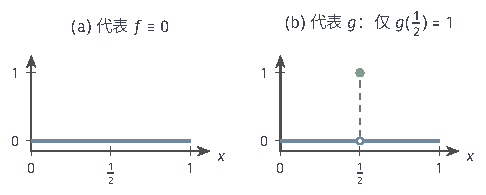
\includegraphics[width=82.2mm]{figures/02-abstract-mathematics/03-function-spaces/tikz/c1-ae-representatives/figure.pdf}
  \caption{同一个几乎处处等价类的两个代表。定义域为$[0,1]$并取Lebesgue测度；(a)中$f\equiv0$，(b)中$g$只在$x=\tfrac12$处取$1$（绿点），空心圈表示$g$在该点不取$0$。单点集测度为零，所以$\int_0^1|f-g|\,dx=0$，二者代表同一个积分空间元素，但它们在$\tfrac12$处的点值不同。}
  \label{fig:fs-ae-representatives}
\end{figure}

\paragraph{等价类与线性运算}
在测度空间$(X,\mathcal A,\mu)$上，对两个可测函数规定
\[
 f\sim_\mu g\quad\Longleftrightarrow\quad \mu(\{x:f(x)\neq g(x)\})=0,
\]
即$f=g$在$\mu$下几乎处处成立。这是一个等价关系：自反与对称是显然的；若$f\sim_\mu g$且$g\sim_\mu h$，则$\{f\neq h\}\subseteq\{f\neq g\}\cup\{g\neq h\}$，两个零测集的并仍是零测集，所以$f\sim_\mu h$。把与$f$几乎处处相等的可测函数全体记为$[f]_\mu$，称为$f$的\term{等价类}（equivalence class），$f$称为它的一个代表。

等价类之间的线性运算借助代表定义：$[f]_\mu+[g]_\mu=[f+g]_\mu$，$c[f]_\mu=[cf]_\mu$。要使这个定义有意义，结果必须不依赖代表的选择。若$f'\sim_\mu f$、$g'\sim_\mu g$，则
\[
 \{f'+g'\neq f+g\}\subseteq\{f'\neq f\}\cup\{g'\neq g\},
\]
右边是零测集，所以$f'+g'\sim_\mu f+g$；数乘同理。于是可测函数的等价类组成一个线性空间，零元素是“几乎处处为零的函数”这一整类。第~\ref{sec:fs-integral}节的$L^p$空间就建立在这样的等价类上。

\paragraph{点值不再自动有意义}
取等价类的代价是：一个类通常没有确定的点值。在Lebesgue测度下每个单点都是零测集，同一类中的代表可以在任意给定的点取任意值，所以“$[f]_\mu$在$x_0$处的值”没有意义。这与测度有关。若某点是原子，即$\mu(\{x_0\})>0$，则同一类的所有代表在$x_0$处必须取同一个值；在计数测度下只有空集是零测集，等价类退化为普通函数。

也不能把等价类当作已经选好了“最好的”代表。在区间上的Lebesgue测度下，若一个类含有连续代表，这个连续代表是唯一的：两个连续函数之差不为零的点组成开集，非空开区间的测度为正，所以两个几乎处处相等的连续函数必定处处相等。但许多类根本没有连续代表（第~\ref{sec:fs-norms-completeness}节的阶跃函数就是一例），而且即使有，从类中读出它的点值也需要另外的论证。本章只固定元素的含义；点值读取何时有良定义、何时连续，由第~\ref{sec:lfo-point-evaluation}小节讨论，点值读取连续的Hilbert函数空间则是第~\ref{chap:rkhs}章的对象。
